%! Author = phili
%! Date = 25/06/2021

\section{Secure Software Lifecycle}
\textbf{SW Engineering processes:} Waterfall, Spiral, Prototyping, XP, Adaptive Programming, ...\\
None of these really support security.\\

\subsection{Software Engineering \& Security}
\begin{itemize}
    \item Often ad hoc or not covered at all
    \item Issues:
    \begin{itemize}
        \item Non systematic approach
        \item Bad early decisions
        \item Hard to manage and modify
    \end{itemize}
\end{itemize}
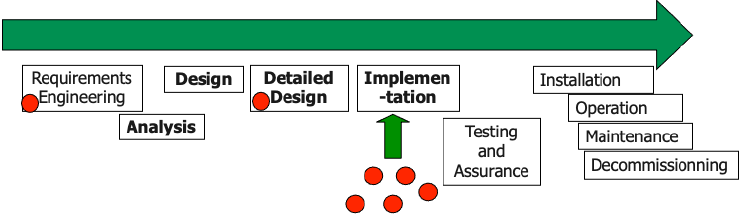
\includegraphics[width=\linewidth]{../img/sw_engineering_security.png}

\subsection{Requirements / Analysis}
\begin{itemize}
    \item Identify security requirements
    \item Quantify the security risks
    \item Know the entire problem domain of the system
\end{itemize}

\subsubsection{Identify Security Requirements}
\begin{enumerate}
    \item Identify stakeholders
    \item Identify assets from different stakeholders (sensitive info / resources)
    \item Identify requirements on these assets
\end{enumerate}
\textbf{Result:} high-level security policy\\
\textbf{STRIDE:} Systematic approach for threat identification.
\begin{itemize}
    \item \textbf{S}poofing
    \item \textbf{T}ampering
    \item \textbf{R}epudiation
    \item \textbf{I}nformation disclosure
    \item \textbf{D}enial of service
    \item \textbf{E}levation of privilege
\end{itemize}

\subsubsection{Quantify Security Risks}
\begin{itemize}
    \item Estimate and quantify the risk of the previously identified threats
    \begin{enumerate}
        \item Importance or severity (critical vs. non-critical)
        \item Cost
        \item DREAD (Damage potential, Reproduceability, Exploitability, Affected users, Discoverability)
    \end{enumerate}
    \item Order the requirements and identify the relevant subset: Risk mitigation strategy
\end{itemize}
\textbf{Result:} high-level security policy revisited

\subsubsection{Example}
\textbf{General formulated:}\\
\textit{The software must validate all user input to ensure it does not exceed the size specified fot that type of input.}\\
\textit{The system must encrypt sensitive data transmitted over the Internet between the server and the browser.}\\
\textbf{Non-functional requirements:}\\
\begin{enumerate}
    \item \textbf{Security Property Requirement}: specifies the characteristics that software must exhibit.
    \item \textbf{Constraint or Negative Requirements} limit what software functionality can be allowed to behave.
    \item \textbf{Security Assurance Requirements} are rules or best practices by which the software security functions will be built, deployed and operated.
\end{enumerate}

\subsection{Detailed Design}
\textbf{Main goals:}\\
\begin{enumerate}
    \item Identify security technologies that meet relevant security requirements
    \item Bind these technologies to the application
\end{enumerate}

\subsubsection{Identify security technologies}
\begin{itemize}
    \item Select requirements that should be addressed at this level
    \item Identify security technologies that address requirements
\end{itemize}
\textbf{STRIDE Countermeasures:}
\textbf{Tampering}
\begin{itemize}
    \item Use data hashing and signing
    \item Digital signatures
    \item Strong authorization
    \item Tamper-resistant protocols across communication links
    \item Secure communication links with protocols that provide message integrity
\end{itemize}
\textbf{Information Disclosure}
\begin{itemize}
    \item Strong authorization
    \item Strong encryption
    \item Secure communication links with protocols that provide message confidentiality
    \item Do not store secrets in plaintext
\end{itemize}
...

\subsubsection{Bind Technologies to Application}
\begin{itemize}
    \item For coarse-grained or simple requirements
    \begin{itemize}
        \item Countermeasure can be realized in the operating system/middleware (SSL)
    \end{itemize}
    \item For fine-grained and complex requirements
    \begin{itemize}
        \item Implement as part of the application (hard to get right)
    \end{itemize}
\end{itemize}

\subsection{Other phases}
\begin{itemize}
    \item Avoiding implementation vulnerabilities
    \item Security testing
    \item Automated patching
\end{itemize}

\subsection{Case study: Web Applications}
\subsubsection{High level Architecture}
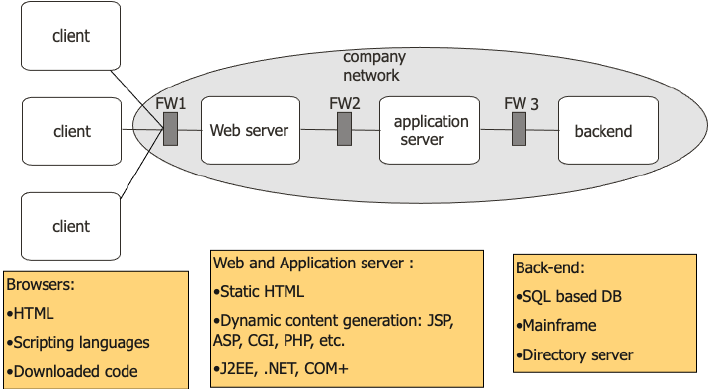
\includegraphics[width=\linewidth]{../img/web_application.png}
\subsubsection{Owners and Assets}
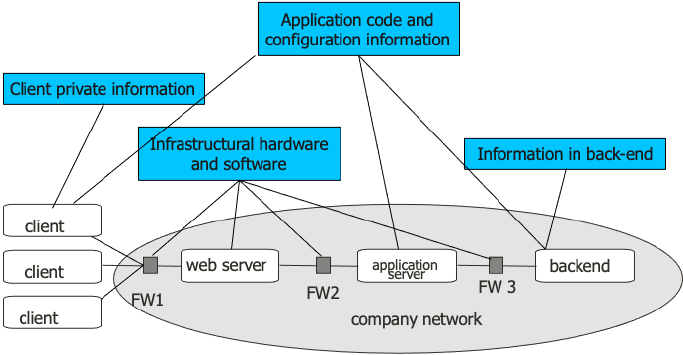
\includegraphics[width=\linewidth]{../img/web_application_owners_assets.png}
\subsubsection{Threat Agents and Threats}
\textbf{Any hacker on the internet:}
\begin{itemize}
    \item Spoof client or server
    \item Eavesdrop on connections / modify data in transit
    \item Bring down infrastructure components
    \item Gain unauthorized access to application or data
\end{itemize}
\textbf{Authorized user of the application: (additionally)}
\begin{itemize}
    \item Repudiate transactions
    \item Elevate privilege
\end{itemize}
\textbf{Malicious server:}
\begin{itemize}
    \item Steal private client information
    \item Spread spyware/viruses
\end{itemize}

\subsubsection{Infrastructural countermeasures}
\textbf{Authentication:}
\begin{itemize}
    \item Network level: IPSEC
    \item Transport level: HTTP authentication mechanisms
    \item OS level: Windows authentication
    \item Single sing-on systems based on federation or windows active directory (Kerberos)
    \item Web authentication products: IAM products
\end{itemize}
\textbf{Data protection:}
\begin{itemize}
    \item IPSEC (Network)
    \item Kerberos (OS)
    \item TLS (Transport)
\end{itemize}
\textbf{Access control:}
\begin{itemize}
    \item Firewall
    \item In the webserver (URL)
    \item RBAC in the web container or application server
    \item File system based access control
    \item Access control products
\end{itemize}
\textbf{Sandboxing:}
\begin{itemize}
    \item At the OS level: low-privileged accounts
    \item Language level: Java security architectures
\end{itemize}
\textbf{Others:}
\begin{itemize}
    \item Filtering
    \item Throttling
    \item Shielding
    \item ...
\end{itemize}

\subsubsection{Typical vulnerabilities}
\textbf{Bugs in functional parts}
\begin{itemize}
    \item Input validation
    \item Race conditions
    \item Bad error handling
\end{itemize}
\textbf{Broken countermeasures}
\begin{itemize}
    \item Access control
    \item Authentication
    \item Crypto
\end{itemize}

\subsubsection{Available Countermeasures at coding level}
\begin{itemize}
    \item Security technologies
    \item Quality improvements
    \begin{itemize}
        \item Choice of programming language
        \item Coding guidelines
        \item Source code scanners
        \item Security testing and audit
        \item Code review
    \end{itemize}
\end{itemize}

\subsection{Daily Sins}
\begin{enumerate}
    \item Buffer Overruns
    \item Format String problems
    \item Integer Overflows
    \item SQL Injection
    \item Command Injection
    \item Failing to Handle Errors
    \item XSS
    \item Failing to protect Network traffic
    \item Use of magic URLs and Hidden Forms
    \item Improper use of SSL and TLS
    \item Use of Weak Password-Based systems
    \item Failing to store and protect data securely
    \item Information leakage
    \item Improper file access
    \item Trusting Network Name Resolution
    \item Race Conditions
    \item Unauthenticated Key Exchange
    \item Cryptographically strong random numbers
    \item Poor usability
\end{enumerate}